\documentclass{uwstat572}

\usepackage{graphicx}
\usepackage{float}
\usepackage{natbib}
\usepackage{amsmath}

%%\setlength{\oddsidemargin}{0.25in}
%%\setlength{\textwidth}{6in}
%%\setlength{\topmargin}{0.5in}
%%\setlength{\textheight}{9in}

\renewcommand{\baselinestretch}{1.5} 


\bibliographystyle{apalike}

\begin{document}
%%\maketitle

\begin{center}
  {\LARGE Statistical Inference and Computational Efficiency for Spatial Infectious Disease Models with Plantation Data}\\\ \\
  {Nathan Welch \\ 
    Department of Statistics, University of Washington Seattle, WA, 98195, USA
  }
\end{center}

\begin{abstract}
This report examines the findings published in \textit{Statistical inference and computational efficiency for spatial infectious disease models with plantation data} \citet{Brown}. 
This paper aims to conduct statistical inference for parameters associated with a simple individual level infectious disease model. 
Model parameters are estimated using the Metropolis sampling algorithm; however, the computation burden created by fitting even a simple model leads to prohibitively long computation time. 
Statistical and computational methods to overcome the computing challenge are reviewed as a result. 
\end{abstract}

\section{Introduction}

Disease propagation modeling is an expansive and active area of mathematical research.
Statistical inference for parameters underlying these models is less mature, but computational advances in recent years make it possible to encode convoluted dependencies and draw inference on the parameters influencing disease propagation. 
Improving our understanding of these parameters will lead to more effective responses or interventions to disease outbreaks. 

\citet{Brown} set out to conduct statistical inference for a simple class of disease propagation models by estimating the risk that a susceptible individual contracts a disease from an infected member of the population. 
In these models, the risk of contracting the disease is modeled at the individual level rather than for the population as a whole. 
The goal is to formulate models that reflect changes in individual risk that correspond to the number of the infected individuals, their proximity to susceptible members of the population, and the duration a susceptible individuals  exposure to those infected. 
While this model is conceptually convenient, the computational complexity and limitations of algorithms capable of fitting such a model create significant challenges.
In \citet{Brown}, the authors appeal to standard likelihood methods and the Metropolis algorithm to estimate a simple individual level model (ILM) for disease propagation.
The emphasis on basic components like the Metropolis sampler and simple disease model focuses readers on common challenges inherent with data for statistical inference with disease data. 

\subsection{Literature Review}
\citet{Haber} introduced ILMs in the context of disease spread among members within households. 
This early ILM assumes infected individuals are dispersed evenly throughout the population. 
It also assumes complete data are available to fit these early models. 
\citet{Becker} surveys a number of models and the types of data sets these models can accommodate. 
His work highlights the distinction between studying disease spread from a mathematical perspective as apposed to a statistical inference point of view and summarizes the principle challenges that disease propagation presents to many statistical methods.

\citet{ONeill} builds on the idea that one does not have to choose between parameter inference and mathematical insight. 
In fact, the authors show that a basic Metropolis-Hastings algorithm clears the way for more realistic modeling assumptions and interdependencies. 
\citet{Jewell} provides an updated perspective and outlines several MCMC design patterns for convoluted models.
\citet{Brown} primarily contributes another example of these methods along with computational efficiencies beyond an MCMC framework. 

While improved computation power made it possible to fit more complex statistical disease models, evaluating likelihood functions that include spatio-temporal components becomes challenging when there are more than a few observations. 
As the cost to evaluate the likelihood function grows with the number of observations, the utility of MCMC approaches declines.
\citet{McKinley} proposes Approximately Bayesian Computation (ABC) that avoids calculating the likelihood by generating an approximation to the likelihood function with each pass through an MCMC implementation. 
\citet{Diggle} forgoes the complexity of full likelihood inference and instead appeals to the partial likelihood function to carry out inference for the parameters of interest. 
\citet{Deardon} uses a Taylor series to approximate infection kernel function to make a Bayesian approach computationally practical. 
These methods led to reduced computation times compared to a full MCMC implementation, but each either require either completely observed data or are too closely associated with a particular model to be widely applicable.

\subsection{Statistical Problem}

\citet{Brown}'s work adopts or adapts some portion of the from the previous section.
The authors use these contributions to model an insect infestation in a Guadeloupe sugar cane field over 30 weeks time. 
This data set is useful for showing how inference may proceed even when essential information needed for mathematical modeling and/or statistical inference are unknown or obfuscated. 

Figure \ref{fig:data_plot} summarizes the sugar cane data set. 
The black dots indicate locations of infected plants at the conclusion of the 30 week study period. 
Grey dots indicate the location of plants that were not infected. 
The plot on the right shows the cumulative number of infected plants for each inspection.

\begin{figure}[H]
\centering
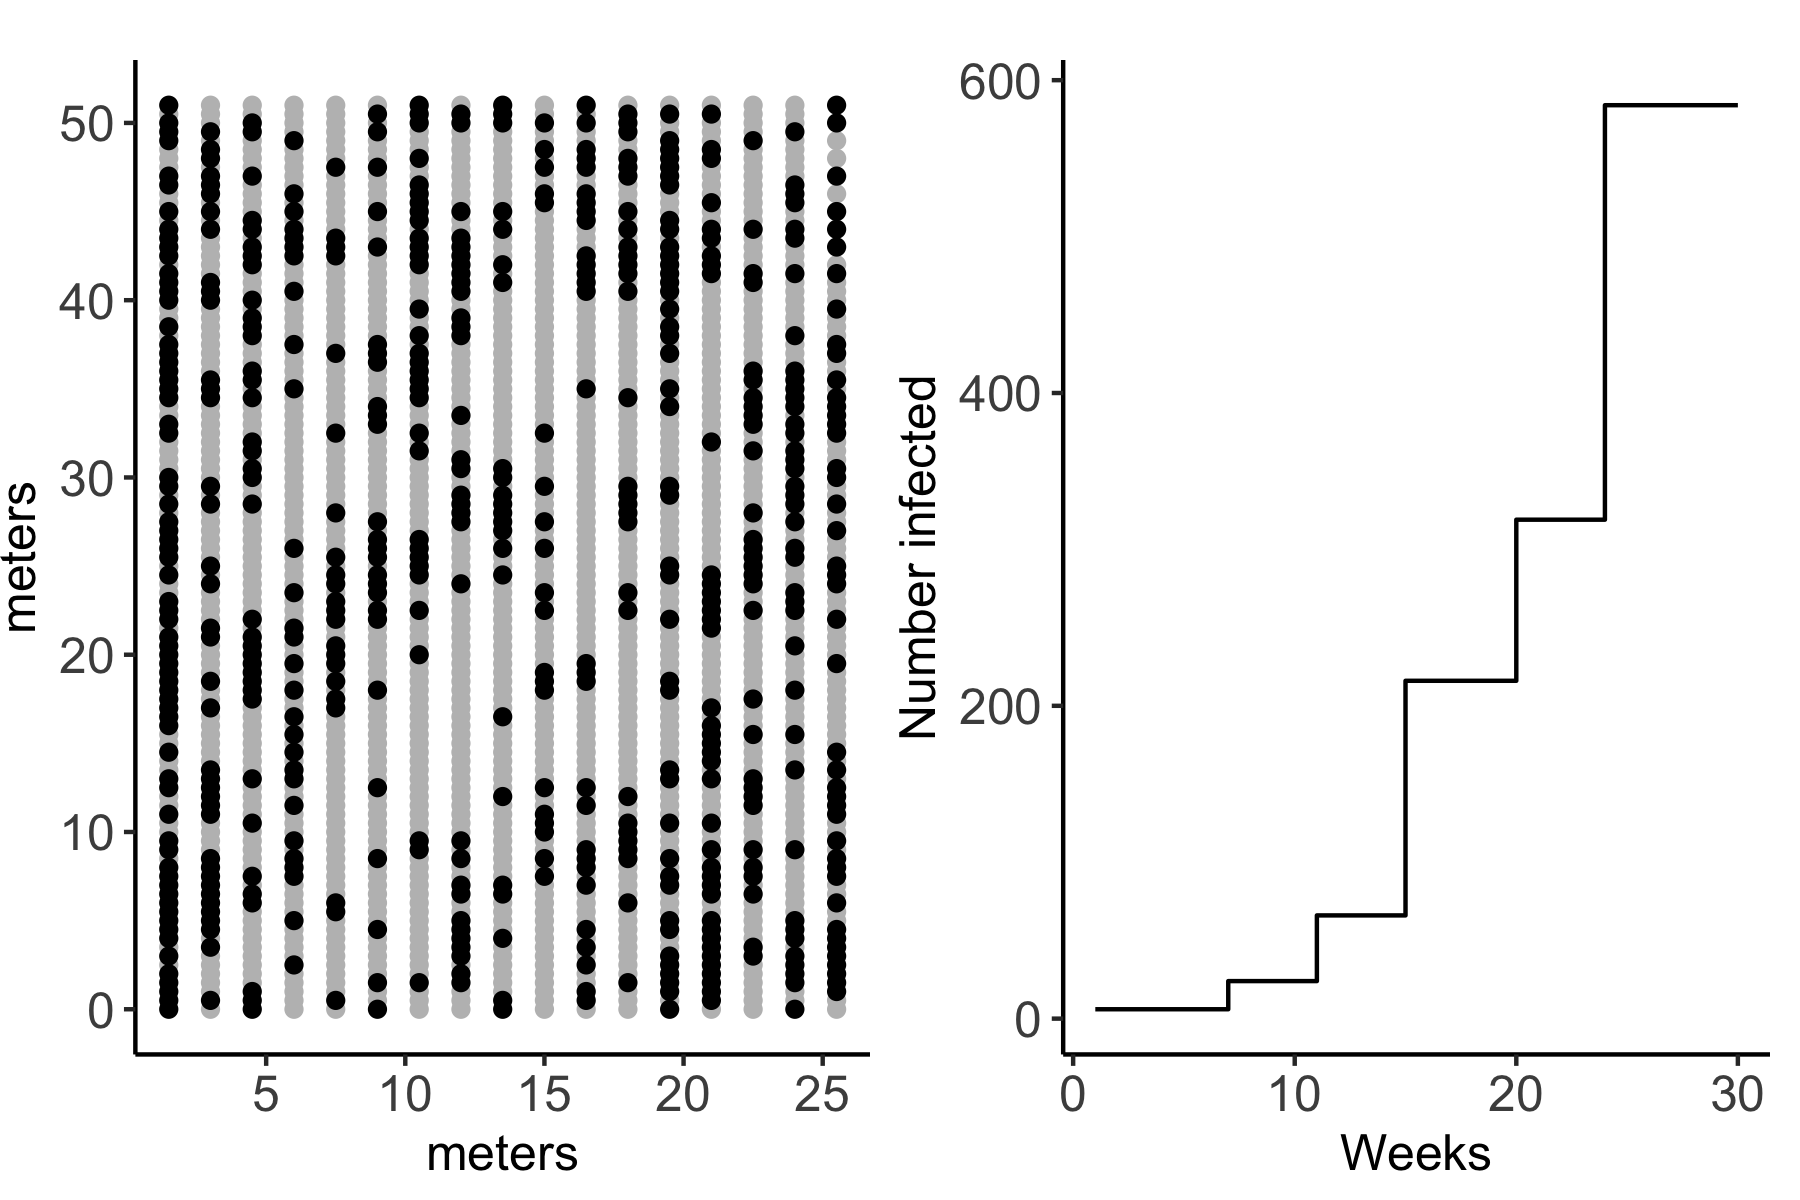
\includegraphics[height=0.5\linewidth, keepaspectratio]{/Users/nwelch/prelim/report/figures/figure_1.png}
\caption{(left) Plant locations (meters) and infection status (black=infected) after 30 weeks; (right) number of infected plants at each inspection time}
\label{fig:data_plot}
\end{figure} 

When modeling disease propagation among individuals who are either susceptible or already infected, the time of infection and duration of susceptible individuals' exposures to infected members of the population are critical. 
These data are necessary to infer the rate at which the disease moves from the infected to the susceptible. 
However, scenarios that include granular infection times are exceptional. 
Such fine detail is typically reserved for extremely dangerous or damaging diseases such as avian flu or foot and mouth disease on farms in developed countries \citep{McKinley}. 
Inference methods for less ominous outbreaks require either additional surveillance, different models, or some other post collection workaround. 

The sugar cane data set includes the infection status of 1,742 plants at six times over a 30 week period. 
Each observation lists the plant location on a two-dimensional rectangular grid and whether it is infected at week 0, 6, 10, 14, 19, 23, and 30.
For this data set, it is reasonable to assume that once a plant becomes infected, it remains infected for the duration of the study period. 
A Susceptible-Infected (SI) model framework is appropriate for this situation and \citet{Jewell} provides a thorough introduction to this and other disease model frameworks. 
While an SI model is particularly simple, the model is plausible considering the way that an infestation proceeds for an aphid infestation of plants over 30 weeks time. 
Starting with a simple model also emphasizes the principle statistical components handled by \citet{Brown}, e.g. unknown infection times. 

Intervals in which susceptible plants became infected are recorded, but the data do not include granular infection time data.  
As a result, there is no way of knowing how long a plant occupied the susceptible and infected stages.
This is a common experimental design, and the details of studies that include this \textit{Type I censoring} with \textit{right} and \textit{interval censored} data are discussed at length in survival analysis texts such as \citet{Klein}. 
While the data collection framework in \citet{Brown} is standard, inference methods for \textit{interval censored} modeling parameters remains more nuanced.

Data augmentation is a common approach to overcoming this inference with unknown infection times. 
In this case, unknown infection times are modeled as latent variables. 
Including these latent variables makes the likelihood function tractable, but inflating the parameter space complicates the model fitting process. 
These factors point to a Bayesian approach to approximating the posterior parameter space of the SI model. 
\citet{Jewell} discusses an augmentation approach in the context of a \textit{Metropolis-in-Gibbs} MCMC framework and the simulation setup described in the next section follows directly. 

\section{Methods}
\subsection{Model and Likelihood}

Inference for ILM model parameters begins with the likelihood function. 
Plausible models account for the locations of infected and susceptible plants along with the respective infection times and durations of exposures. 
However, time intervals in which a susceptible plant becomes infected offer the only temporal queues. 
As a result, lets treat infection time, $\tau_j$, for plant $j$ as a latent variable whose domain is restricted to the period in which the infection status of plant $x_j$ changed. 

The model must also account for the transmission rate differential induced by the physical distance separating infected and susceptible plants. 
The transmission rate between an infected plant far from a susceptible plant should be smaller than the rate between two plants next to one another.
As a result, let the function $\theta f(x_i -x_j \sigma | \sigma)$ dente the rate of infection for plant $i$ at time $t$ and for a plant $j$ infected prior to $t$. 
After including a term capturing the rate of spontaneous infection $\mu$, the hazard function at plant $i$ and time $t$ given the infection times for plants $j \in \{1, 2, \dots, 1742\}$ is 
$$\lambda(x_i,t) = \mu + \sum_{j; \tau_j<t} \theta \, f(x_i - x_j; \sigma)$$
Now consider the contribution that plant $x_i$ makes to the likelihood if it is infected at time $0<\tau_i<T=30$ weeks. 
By definition of the hazard function, the instantaneous infection rate at plant $x_i$ is \textbf{[double check notation]}
\begin{align*}
\lambda(x_i, t) &= \lim_{dt \to 0} \frac{Pr\{ t \le \tau_i < t+dt | \tau_i \ge t \}}{dt} \\
	&= \lim_{dt \to 0} \frac{Pr\{ t \le \tau_i < t+dt\}}{Pr\{\tau_i\ge t\}dt}\\
	&= \lim_{dt \to 0} \frac{F_i(t+dt) - F_i(t)}{(1-F_i(t))dt} \\
	&= \frac{f_i(t)}{S_i(t)}\\
	&= -\frac{d}{dt} \log S_i(t) \\
\implies S_i(t) &= \exp \left\{ - \int_0^t \lambda(x_i,s) ds  \right\} = \exp \left\{ - \Lambda_i(t)  \right\}
\end{align*}
where $S_i$, $f_i$, and $\Lambda_i$ denote the respective survival function, probability distribution function (pdf), and cumulative hazard for plant $x_i$. 
From this expression, it follows that
$$ f_i(t) = \lambda(x_i,t) \exp \left\{ - \int_0^t \lambda(x_i,t) dt  \right\}$$
establishing the pdf that plant $x_i$ contributes to the likelihood function if $t<T=30$ weeks. 
Plants that remain healthy throughout the study period contribute $S_i(t)$ to the likelihood. 
As a result, the likelihood function is
\begin{equation} 
L(\theta, \mu, \tau) = \left[ \prod_{i;\tau_i \le T} \exp \left\{-\int^{\tau_i}_0 \lambda(x_i, t)dt\right \} \lambda(x_i, \tau_i)\right] \left[ \prod_{i;\tau_i > T} \exp \left\{-\int^{\tau_i}_0 \lambda(x_i, t)dt \right\}\right] 
\end{equation}

The last component of the model to specify is the kernel function, $f(x_i -x_j | \sigma)$. 
In this case, a radially symmetric bivariate Gaussian density is appropriate. 
\begin{equation} f( x_i-x_j |\sigma) = \frac{1}{\sqrt{2\pi \sigma^2}} \exp \left\{-\frac{(x_i-x_j )^2}{2\sigma^2} \right\} \label{eq:kernel} \end{equation}
The Gaussian kernel is physically reasonable since the movement of aphids among plants can be modeled by Brownian Motion. 
With this argument, $\sigma^2$ in (\ref{eq:kernel}) denotes the variance of the distance an aphid travels in one week. 

\subsection{Prior Distributions}
Weakly informative priors were used for the endemic infection rate ($\mu$), the epidemic infection rate ($\theta$), and the variance for distance disease travels in a week ($\sigma^2$). 
Prior parameters were specified using 95\% prior prediction intervals for each parameter. 

\textbf{[I worked out the details for $\mu$, and it's ready for writeup. $\theta$ and $\sigma$ are still in process. Everything below is still the first draft/junk...]}

\begin{itemize}
\item $\mu \sim$ Gamma(0.7, 0.004) yields a 95\% prediction interval between 1 and 630. 583 infections were observed in the data.
\item $\theta \sim$ Gamma(0.8, 10) leads to an infected plant requiring 1 to 16 weeks time to produce the first infection when surrounded by susceptible plants
\item $\sigma \sim$ Gamma(0.5, 100) implies that nearly all aphids will have traveled less than 10 cm at the 2.5\% quantile and around 500 meters at the 95.5\% quantile
\end{itemize}
Placing $\mu$ and $\theta$ at the lower end of their ranges leads to few infections over 30 weeks time. 
Setting these too high leads to nearly universal infection. 
Extreme values of $\sigma$ leads a to somewhat different result. 
Specifying $\sigma$ too small would imply that the aphids driving the infection spread are incapable of moving between plants. 
Setting $\sigma$ too large removes the spatial component of the model. 
\citet{Brown} specified priors leading to physically plausible outcomes. 


\subsection{Inference}
Exact infection times, $\tau_i$, are unobserved. 
Only the intervals in which a plant became infected offer clues about the status of plants during the study period. 
Since each plant's infection status and location influence all other plants at each time step, there is no way to eliminate the dependency on the unknown infection times, $\tau$.
\citet{Brown} follows a data augmentation and MCMC approach to resolve handle the issue. 
This process is known as a \textit{non-centering parameterization}.
\citet{Jewell} section 2.2 outlines a modeling framework nearly identical to the methods followed here. 

In this case, priors are specified for the model parameters of interest, specifically $\theta$, $\sigma$, and $\mu$. 
Infection intervals, $\textbf{Y} = \{Y_i:i=1,\dots, N\}$, are the data. 
The Metropolis algorithm summarized below leads to a posterior sample from $\pi(\mu, \theta, \sigma, \tau \mid \textbf{Y})$. 

\begin{enumerate}
\item Initialize the algorithm at $\tau_i^{0}$, $\mu^{0}$, $\sigma^{0}$, $\theta^{0}$ for iteration $r=0$
\item at iteration $r$, set $\tau_i^{(r)}=\tau_i^{(r-1)}$, $\mu^{(r)}=\mu^{(r-1)}$, $\sigma^{(r)}=\sigma^{(r-1)}$, $\theta^{(r)}=\theta^{(r-1)}$
\item simulate a proposal $\mu^{\star} \sim N(\mu^{(r-1)}, \nu_{\mu})$
\item set $\mu^{(r)} = \mu^{\star}$ with probability
$$\min \left\{1, \frac{L( \tau^{(r)}_1, \dots, \tau^{(r)}_N \mid \mu^{\star}, \theta^{(r)}, \sigma^{(r)} ) \; p_{\mu}(\mu^{\star})}{L(\tau^{(r)}_1, \dots, \tau^{(r)}_N \mid \mu^{(r)}, \theta^{(r)}, \sigma^{(r)} ) \; p_{\mu}(\mu^{r})} \right\} $$
			otherwise, set $\mu^{(r)}=\mu^{(r-1)}$
\item repeat steps 3 and 4 for $\theta$ and $\sigma$
\item for each $i=1, \dots, N$, propose a new $\tau^{\star}_i$ and accept with probability
$$\min \left\{1, \frac{L( \tau^{(r)}_1, \dots, \tau^{(r)}_{i-1}, \tau^{\star}_i,\tau^{(r)}_{i+1}, \dots, \tau^{(r)}_N \mid \mu^{(r)}, \theta^{(r)}, \sigma^{(r)} ) \; p_{\mu}(\mu^{\star})}{L(\tau^{(r)}_1, \dots, \tau^{(r)}_N \mid \mu^{(r)}, \theta^{(r)}, \sigma^{(r)} ) \; p_{\mu}(\mu^{r})} \right\} $$
\item return to step 2 until a sufficiently large sample has been obtained
\end{enumerate}

The implementation for this model uses normally distributed proposals with means at the previous $\theta$, $\sigma$, $\mu$, and $\tau_i$ values and $ \nu_{\theta}=0.005^2$, $ \nu_{\mu}=0.0005^2$, $ \nu_{\sigma}=0.05^2$, and $ \nu_{\tau^{(r)}_i}=1$. 
The authors select these standard deviations after assessing the mixing properties of test runs. 

\subsection{Implementation}
The data include 583 unknown infection times. 
As a result, some portion of the likelihood function has to be computed 586 times for each pass through the sampler. 
Implementing the algorithm naively leads to prohibitively long computation times. 
The following sections review the steps taken to improve and benchmark computational performance enough to make the non-centering parameterization method viable for data with challenging interdependencies. 
The methods were implemented in the Julia. 

\subsubsection{Basic Algorithm}
The basic implementation primarily executes the pseudo-code from the previous section with three exceptions.
First, the distance matrix among the 1,742 plants is pre-computed and referenced throughout the implementation. 
The other exception concerns the $\tau^{(r)}$ update routine. 
Many of the terms in the likelihood ratio are identical, eliminating the need to compute several terms in the likelihood function. 
Finally, eliminating impossible infection time sequences among the remaining pieces of the computation led to efficiencies in the compute time.

\subsubsection{Parallel Algorithm}
The parallel implementation distributes the computational burden two different ways. 
Both focus on computing updating $\tau$. 
First, the subroutines of the likelihood ratio that cannot run asynchronously but still require significant computational resources are broken into pieces and computed on multiple cores. 
The other parallelization improvement results from recognizing that some updates are not possible given order that infections were known to have occurred. 
As a result, proposals that would reverse this known ordering are rejected immediately. 
More to come... 

\subsubsection{Improved Parallel Algorithm}
Tbd...

\subsubsection{Truncated Algorithm}
Tbd...

\subsubsection{Discrete Time Algorithms}
Tbd...

\section{Results}

\section{Discussion}

\bibliography{/Users/nwelch/prelim/report/prelim_references}

\end{document}









